% do Greedy proofs too if you have time
\section*{Divide and Conquer}
\begin{itemize}
    \item Summations and Geometric Series 
    % \\
    % 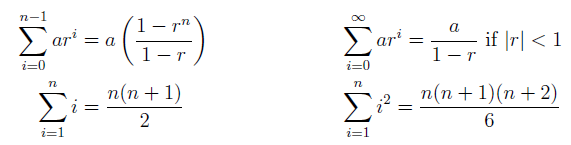
\includegraphics[scale = 0.75]{pictures/summation.png}
\end{itemize}
{\color{Violet}
\begin{align*}
    \sum^{n}_{i=1} a r^i &= a \left(\frac{1-r^n}{1-r} \right) = a\cdot   \frac{r^{n+1}-1}{r-1}
    &&\sum_{i=0}^\infty ar^i = \frac{a}{1-r} ~~~ \text{ if } |r| < 1 \\
    \sum^n_{i=1} i &= \frac{n(n+1)}{2} 
    &&\sum^n_{i=1}i^2 = \frac{n(n+1)(n+2)}{6}
\end{align*}
}
\begin{itemize}
    \item \ul{\textbf{The Master Theorem}}
    {\color{Violet}
    \begin{align*}
        T(n) &= 
        \begin{cases}
            c~ \text{ (has to be constant)} &\text{if } n < n_0 \\
            aT\left(\frac{n}{b} \right) + cn^k &\text{if } n \geq n_0
        \end{cases} \\
        \text{if } a > b^k &: T(n) \in \Theta(n ^{\log_b a}) \\
        \text{if } a = b^k &: T(n) \in \Theta(n^k \log n) \\
        \text{if } a < b^k &: T(n) \in \Theta(n^k)
    \end{align*}
    }
    $\rightarrow$ Master theorem does not always give same bound as tree
    \item let tree be $T(n) = a T(n/b) + cn$, then $height(tree) = \log_b n$
    \item some divide and conquer algo w/ their runtime\\
    $\longrightarrow$ quickSort: $\Theta(n\log n )$\\
    $\longrightarrow$ quickSelect (find k-th largest element in array): $\Theta(n)$
    \item find work per level: get work at level one in form of $cn^k \cdot (a/b)$ and the work per level is $cn^k(a/b)^i$
    \item if you can't use Master theorem (unequal split) - 2 ways 
    \begin{itemize}[leftmargin = 1em]
        \item \ul{\textbf{massage into Master Theorem}}: 
            \begin{align*}
                T(n) &= T\left( \frac{3n}{4} \right) + T \left(\frac{n}{8} \right) + cn \\
                \text{define } L(n) &= T \left(\frac{n}{8} \right) + T \left(\frac{n}{8} \right) + cn \leq T(n) \\
                &= 2T \left(\frac{n}{8} \right) + cn  \\
                U(n) &= 2 T \left(\frac{3n}{4} \right) +cn \geq T(n) \\ 
                \text{via Master, } L(n) &= \Theta(n) \therefore T(n) = \Omega(n) \\ 
                U(n) &= \Theta(n) \therefore T(n) = O(n) \\
                \therefore T(n) &= \theta(n)
            \end{align*}
        \item \ul{\textbf{take sum to infinity}}: the lower bound is the work done at level 0, and upper bound is sum of work done per level take to infinity 
        \begin{itemize}[leftmargin = 1em]
            \item usually give tighter bound than the Master Theorem
            \item ex. $T(n) = 2T(n/3) + T(n/4) + cn^2$ for $n > 3$, constant other wise \\
            Work done at level 0: one root node of size n with time $cn^2$ \\
            Work done at level 1:
            \[c(n/3)^2 + c(n/3)^2 + c(n/4)^2 = cn^2(41/144)\] 
            Work per level: $cn^2 \cdot (41/144)^i$ \\
            Lower bound: work done at level 0 so lower bound is $ \Omega(cn^2)$\\
            Upper bound: 
            \begin{align*}
                \sum^\infty_{i=1} cn^2 \left(\frac{41}{144} \right)^i &= \dfrac{cn^2}{1-\frac{41}{144}} = cn^2 \left(\frac{103}{144} \right) = O(n^2)
            \end{align*}
        \end{itemize}
        
    \end{itemize}
\end{itemize}

